%----------------------------------------------------------------------------------------
%	PACKAGES AND OTHER DOCUMENT CONFIGURATIONS
%----------------------------------------------------------------------------------------
\documentclass[12pt]{article}
\usepackage{graphicx}
\usepackage{amsmath,amsfonts,stmaryrd,amssymb} % Math packages
\usepackage{bm}
\usepackage{steinmetz}
\usepackage{enumitem}
\graphicspath{{images/}}
\usepackage{float}
\usepackage{hyperref}
\hypersetup{
	colorlinks=true,
	linkcolor=blue,
	filecolor=magenta,      
	urlcolor=cyan,
	pdftitle={Overleaf Example},
	pdfpagemode=FullScreen,
}
\urlstyle{same}
\usepackage{mathtools}
\usepackage{fancyhdr}
\usepackage{xcolor}
\usepackage[american,RPvoltages]{circuiTikz}
\usepackage{tikz, tikz-cd}
\usepackage{pgfplots}
\usepackage{siunitx}
\usetikzlibrary{spy,shapes,arrows, arrows.meta, bending, decorations.markings}
\pgfplotsset{width=10cm,compat=1.18}
\usepackage{lmodern} % package for changing font size
\usepackage{lastpage}
\renewcommand{\figurename}{Figura}
\usepackage{tcolorbox}
\usepackage{lipsum}
%\usepackage{enumerate} % Custom item numbers for enumerations
\usepackage[ruled]{algorithm2e} % Algorithms
\usepackage[framemethod=tikz]{mdframed} % Allows defining custom boxed/framed environments
\usepackage{listings} % File listings, with syntax highlighting
%\lstset{basicstyle=\ttfamily,} % Typeset listings in monospace font
\usepackage{lipsum}
\tcbuselibrary{listings,theorems,skins,vignette,raster,breakable,magazine,poster,fitting,hooks}
\usepackage[T1]{fontenc}
\usepackage{tgbonum}
 \fontfamily{garamond}
\definecolor{myblue}{RGB}{24, 51, 73}
%----------------------------------------------------------------------------------------
%	DOCUMENT MARGINS
%----------------------------------------------------------------------------------------

\usepackage{geometry} % Required for adjusting page dimensions and margins
\geometry{
	paper=a4paper, % Paper size, change to letterpaper for US letter size
	top=2.5cm, % Top margin
	bottom=3cm, % Bottom margin
	left=2cm, % Left margin
	right=2.5cm, % Right margin
	headheight=14pt, % Header height
	footskip=1.5cm, % Space from the bottom margin to the baseline of the footer
	headsep=1.2cm, % Space from the top margin to the baseline of the header
	%showframe, % Uncomment to show how the type block is set on the page
}

%----------------------------------------------------------------------------------------
%	FONTS
%----------------------------------------------------------------------------------------

\usepackage[utf8]{inputenc} % Required for inputting international characters
\usepackage[T1]{fontenc} % Output font encoding for international characters
\usepackage{XCharter} % Use the XCharter fonts
\usepackage{tgbonum}

\makeatletter
\pgfcircdeclarebipole{}{\ctikzvalof{bipoles/vsourcesin/height}}{sVpm}{\ctikzvalof{bipoles/vsourcesin/height}}{\ctikzvalof{bipoles/vsourcesin/width}}{
	
	\pgfsetlinewidth{\pgfkeysvalueof{/tikz/circuitikz/bipoles/thickness}\pgfstartlinewidth}
	\pgfpathellipse{\pgfpointorigin}{\pgfpoint{0}{\pgf@circ@res@up}}{\pgfpoint{\pgf@circ@res@left}{0}}
	\pgfusepath{draw}     
	\pgftext[bottom,rotate=90,y=\ctikzvalof{bipoles/vsourceam/margin}\pgf@circ@res@down]{\scriptsize$-$}
	\pgftext[top,rotate=90,y=\ctikzvalof{bipoles/vsourceam/margin}\pgf@circ@res@up]{\scriptsize$+$}
	
	\pgf@circ@res@up = .35\pgf@circ@res@up
	\pgfscope
	\pgftransformrotate{90}
	\pgfpathmoveto{\pgfpoint{-\pgf@circ@res@up}{0cm}}
	\pgfpathsine{\pgfpoint{.5\pgf@circ@res@up}{.4\pgf@circ@res@up}}
	\pgfpathcosine{\pgfpoint{.5\pgf@circ@res@up}{-.4\pgf@circ@res@up}}
	\pgfpathsine{\pgfpoint{.5\pgf@circ@res@up}{-.4\pgf@circ@res@up}}
	\pgfpathcosine{\pgfpoint{.5\pgf@circ@res@up}{.4\pgf@circ@res@up}}
	\pgfusepath{draw}
	\endpgfscope
}
\def\pgf@circ@sVpm@path#1{\pgf@circ@bipole@path{sVpm}{#1}}
\compattikzset{sinusoidal voltage source pm/.style = {\circuitikzbasekey, /tikz/to path=\pgf@circ@sVpm@path, \circuitikzbasekey/bipole/is voltage=true, \circuitikzbasekey/bipole/is voltageoutsideofsymbol=true, v=#1 }}
\compattikzset{sVpm/.style = {\comnpatname sinusoidal voltage source pm = #1}}

\pgfcircdeclarebipole{}{\ctikzvalof{bipoles/vsourcesin/height}}{sVpmh}{\ctikzvalof{bipoles/vsourcesin/height}}{\ctikzvalof{bipoles/vsourcesin/width}}{
	
	\pgfsetlinewidth{\pgfkeysvalueof{/tikz/circuitikz/bipoles/thickness}\pgfstartlinewidth}
	\pgfpathellipse{\pgfpointorigin}{\pgfpoint{0}{\pgf@circ@res@up}}{\pgfpoint{\pgf@circ@res@left}{0}}
	\pgfusepath{draw}     
	\pgftext[center,x=0.2\pgf@circ@res@down-\ctikzvalof{bipoles/vsourceam/margin}\pgf@circ@res@down]{\scriptsize$-$}
	\pgftext[top,rotate=90,y=\ctikzvalof{bipoles/vsourceam/margin}\pgf@circ@res@up]{\scriptsize$+$}
	
	\pgf@circ@res@up = .35\pgf@circ@res@up
	\pgfscope
	\pgftransformrotate{90}
	\pgfpathmoveto{\pgfpoint{-\pgf@circ@res@up}{0cm}}
	\pgfpathsine{\pgfpoint{.5\pgf@circ@res@up}{.4\pgf@circ@res@up}}
	\pgfpathcosine{\pgfpoint{.5\pgf@circ@res@up}{-.4\pgf@circ@res@up}}
	\pgfpathsine{\pgfpoint{.5\pgf@circ@res@up}{-.4\pgf@circ@res@up}}
	\pgfpathcosine{\pgfpoint{.5\pgf@circ@res@up}{.4\pgf@circ@res@up}}
	\pgfusepath{draw}
	\endpgfscope
}
\def\pgf@circ@sVpmh@path#1{\pgf@circ@bipole@path{sVpmh}{#1}}
\compattikzset{sinusoidal voltage source pmh/.style = {\circuitikzbasekey, /tikz/to path=\pgf@circ@sVpmh@path, \circuitikzbasekey/bipole/is voltage=true, \circuitikzbasekey/bipole/is voltageoutsideofsymbol=true, v=#1 }}
\compattikzset{sVpmh/.style = {\comnpatname sinusoidal voltage source pmh = #1}}
\makeatother


%----------------------------------------------------------------------------------------
%	BEGIN DOCUMENT
%----------------------------------------------------------------------------------------

\begin{document}
	%\thispagestyle{empty}
	\begin{tikzpicture}[remember picture, overlay]
		\node[anchor=north west, inner sep=0pt] at (current page.north west) {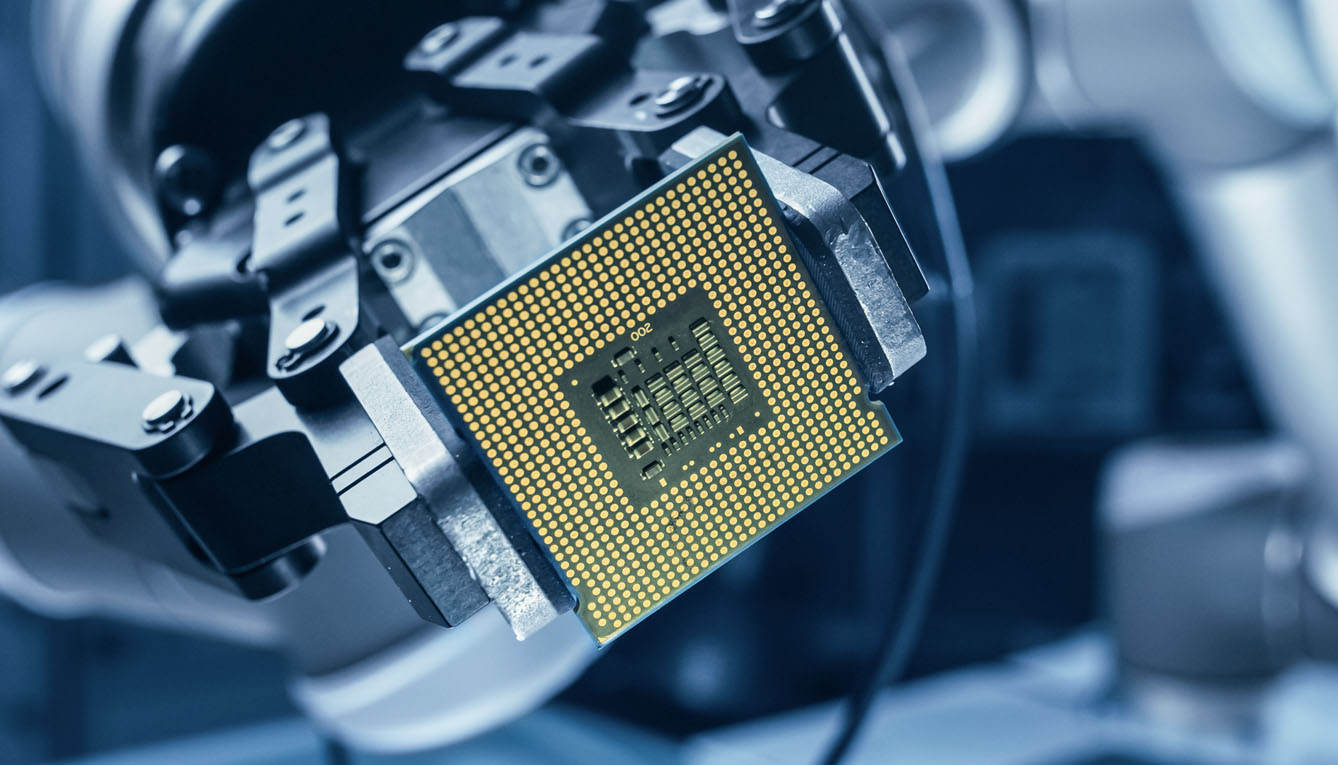
\includegraphics[width=\paperwidth, height=.5\paperheight]{picture1}};
	\end{tikzpicture}

	\vspace{13cm}
	\noindent \textcolor{myblue}{\fontsize{40pt}{40pt}\selectfont \textbf{Fuente de corriente Widlar}}\\\\\\
	{\fontsize{18pt}{18pt}\selectfont 12 de Agosto del 2023} 
	
	\newpage
	\section*{Fuente de corriente Widlar}
	El espejo de corriente básico tiene una limitación. Cada que necesitemos un valor de corriente bajo, el valor de la resistencia $R_1$ requerida debe ser lo suficientemente alta pero tiene la limitación de que no puede ser fabricada económicamente en circuitos IC's. La figura 1 muestra el espejo de corriente Widlar el cual es particularmente apropiado para valores bajos de corriente. El circuito difiere del espejo de corriente básico sólo en la resistencia $R_E$ que está incluida en la terminal de emisor del transistor $Q_2$.  
	
	
	\begin{figure}[H]
		\centering	
		\begin{tikzpicture}[scale=0.8]
			\draw (0,0) node[npn, xscale=-1](Q1){};
			\coordinate (M) at ($(Q1.C)!0.5!(Q1.E)$);
			\draw (M) node[left]{$Q_1$};
			\draw (Q1.B) to[short] ++(4,0) coordinate(node1);
			\draw (node1) node[npn, right](Q2){$Q_2$};
			\coordinate (M1) at ($(Q1.B)!0.5!(Q2.B)$);
			\draw (Q1.C) to[short, f<=$I_C$] ++(0,1) coordinate(node2);
			\draw (node2) to[R, l=$R_1$, f<=$I_{ref}$] ++(0,3) coordinate(node3) node[vcc]{$V_{CC}$};
			\draw (node2) to[short, *-] (node2 -| M1) -- (M1);
			\draw (M1) to[short, *-] (M1);
			\draw (Q2.C) to[short, f<_={$I_{C2} = 0$}] (Q2.C |- node3);
			\draw (Q1.B) to[short, f<=$I_{B1}$] (M1);
			\draw (M1) to[short, f=$I_{B2}$] (Q2.B);
			\draw (Q2.E) to[R, l_=$R_E$, f>^={$I_{B2} + I_{C2}$}] ++(0,-3) coordinate(node4);
			\draw (Q1.E) to[short] ++(0,-3) coordinate(node5); 
			\draw (node4) to[short] (node5);
			\coordinate (M2) at ($(node4)!0.5!(node5)$);
			\draw (M2) node[ground]{};
			\draw (M2) to[short, *-] (M2);
			\draw (Q1.B) node[below, xshift=0.2cm]{$+$};
			\draw (Q1.E) node[right, yshift=-0.3cm]{$-$};
			\draw (Q1.B) node[xshift=0.1cm, yshift=-0.75cm]{$V_{BE1}$};
			\draw (Q2.B) node[below, xshift=-0.2cm]{$+$};
			\draw (Q2.E) node[left, yshift=-0.3cm]{$-$};
			\draw (Q2.B) node[xshift=-0.1cm, yshift=-0.75cm]{$V_{BE2}$};
		\end{tikzpicture}
		\caption{Amplificador multietapa}	
		\label{fig:figura1}
	\end{figure}
	
	\noindent Es posible observar que debido a la resistencia $R_E$ el voltaje base-emisor $V_{BE2}$ es menor que $V_{BE1}$ y consecuentemente la corriente $I_O$ será menor que la corriente $I_{C1}$.
	
	\noindent La corriente de colector $I_{C1}$ e $I_{C2}$ de los transistores $Q_1$ y $Q_2$ puede expresarse aproximadamente como
	\begin{align}
		I_{C1} = \alpha_F I_{ES}\exp \left( \frac{V_{BE1}}{V_T} \right) \\
		I_{C2} = \alpha_F I_{ES}\exp \left( \frac{V_{BE2}}{V_T} \right)
	\end{align}
	
	\noindent La relación entre las corrientes de colector $I_C1$ e $I_{C2}$ usando las ecuaciones (1) y (2) está dada por
	\begin{align}
		\frac{I_{C1}}{I_{C2}} = \exp \left( \frac{V_{BE1} - V_{BE2} }{V_T} \right)
	\end{align}
	
	\noindent Tomando el logaritmo natural en ambos lados de la ecuación (3) obtenemos
	\begin{align*}
		\ln \left( \frac{I_{C1}}{I_{C2}} \right) = \ln\left( e^{\frac{ V_{BE1} - V_{BE2} }{V_T}} \right)\\
		\ln \left( \frac{I_{C1}}{I_{C2}} \right) = \frac{V_{BE1} - V_{BE2}}{V_T}
	\end{align*}
	
	\begin{align}
		V_{BE1} - V_{BE2} = V_T \ln \left( \frac{I_{C1}}{I_{C2}} \right)
	\end{align}
	
	\noindent Al emplear la LTK en el lazo inferior obtenemos
	\begin{align*}
		V_{BE1} - V_{BE2} - R_E (I_{B2} + I_{C2}) = 0\\
		V_{BE1} - V_{BE2} = R_E (I_{B2} + I_{C2})\\
		V_{BE1} - V_{BE2} = R_E \left( \frac{I_{C2}}{\beta} + I_{C2} \right)
	\end{align*}
	
	\noindent O bien
	\begin{align}
		V_{BE1} - V_{BE2} = I_{C2}R_E\left( \frac{1}{\beta} + 1 \right) 	
	\end{align}
	
	\noindent La sustitución de la ecuación (4) en (5) produce
	\begin{align}
		V_T \ln \left( \frac{I_{C1}}{I_{C2}} \right) = I_{C2}R_E\left( \frac{1}{\beta} + 1 \right)
	\end{align}
	
	\noindent Al despejar $R_E$ de la ecuacipon (6) obtenemos
	\begin{tcolorbox}[colback=red!5!white,colframe=red!75!black,arc=0mm,boxrule=0mm,width=(\linewidth+0.5cm)]
		\begin{equation}
			R_E = \frac{V_T}{\left( \frac{1}{\beta} + 1 \right)I_{C2}}\ln \left( \frac{I_{C1}}{I_{C2}} \right)	
		\end{equation}
	\end{tcolorbox}
	
	\noindent La relación entre $I_{C1}$ y la corriente de referencia $I_{ref}$ se obtiene empleando la LCK en el nodo que corresponde a la resistencia $R_1$ y el transistor $Q_1$
	
	\begin{align*}
		I_{ref} = I_{C1} + I_{B1} + I_{B2}\\
		I_{ref} = I_{C1} + \frac{I_{C1}}{\beta} + \frac{I_{C2}}{\beta}
	\end{align*}
	
	\begin{align}
		I_{ref} = I_{C1}\left( 1 + \frac{1}{\beta} \right) + \frac{I_{C2}}{\beta}
	\end{align}
	
	\noindent (Asumiendo que $\beta_1 = \beta2 = \beta$ para transistores idénticos). Además notamos en la ecuación (8) que consta de dos términos, el término $I_{C1}$ multiplicado por un factor de $\left( 1 + \frac{1}{\beta} \right) $ y el término $I_{C2}$ multiplicado por un factor de $\frac{1}{\beta}$. Si asumimos un valor de $\beta=100$ el primer factor sería igual a $\left( 1 + \frac{1}{\beta} \right) = 1.01$ mientras que el segundo factor toma un valor de $\frac{1}{\beta} = 0.01$, por lo que podemos inferir que en la fuente de corriente Widlar $I_{C2}  \ll I_{C1}$. Así el término $\frac{I_{C2}}{\beta}$ puede ser despreciado en la ecuación (8).
	
	\begin{align}
		I_{ref} \cong I_{C1}\left( 1 + \frac{1}{\beta} \right)
	\end{align}
	
	\noindent O
	\begin{tcolorbox}[colback=red!5!white,colframe=red!75!black,arc=0mm,boxrule=0mm,width=(\linewidth+0.5cm)]
		\begin{equation}
			I_{C1} = \frac{\beta}{\beta + 1}I_{ref}
		\end{equation}
	\end{tcolorbox}
	
	\noindent Donde
	\begin{tcolorbox}[colback=red!5!white,colframe=red!75!black,arc=0mm,boxrule=0mm,width=(\linewidth+0.5cm)]
		\begin{equation}
			I_{ref} = \frac{V_{CC} - V_{BE}}{R_1}
		\end{equation}
	\end{tcolorbox}
	
	\noindent Para $\beta \gg 1$
	\begin{align}
		I_{ref} \cong I_{C1}
	\end{align}
	
	\subsection*{Ejemplo}
	Disele una fuente de corriente Widlar para generar una corriente constante $I_o = \SI{10}{\micro\ampere}$. Asuma que $V_{CC} = \SI{10}{\volt}, V_{BE} = \SI{0.7}{\volt}, \beta=125$. Use $V_T = \SI{25}{\milli\volt}$.
	
	
	\noindent Para la fuente de corriente Widlar primero debemos decidir un valor apropiado para $I_ref$. Si escogemos $I_{ref} = \SI{1}{\milli\ampere}$, entonces $R_1$ está dado por
	\begin{align}
		R_1 = \frac{\SI{10}{\volt} - \SI{0.7}{\volt}}{\SI{1}{\milli\ampere}} = \SI{9.3}{\kilo\ohm}
	\end{align}
	
	\noindent El valor de $R_E$ está dado por la ecuación (7)
	\begin{align}
		R_E = \frac{\SI{25}{\milli\volt}}{\left(1 + \frac{1}{125}\right)\SI{10}{\micro\ampere}}\ln \left( \frac{\SI{1}{\milli\ampere}}{\SI{10}{\micro\ampere}} \right) = \SI{11.5}{\kilo\ohm}
	\end{align}
	
	\noindent Es claro ver que el circuito de Widlar permite la generación de constantes pequeñas usando resistores relativamente pequeños.
\end{document}